% !TEX TS-program = pdflatex
% !TEX encoding = UTF-8 Unicode

\documentclass[10pt, a4paper]{article}

% Essential packages
\usepackage[utf8]{inputenc}
\usepackage[T1]{fontenc}
\usepackage{helvet}
\usepackage{amssymb}
\usepackage{graphicx}
\renewcommand{\familydefault}{\sfdefault}

% Page geometry for landscape layout
\usepackage{geometry}
\geometry{a4paper, landscape, margin=1cm, top=1cm, bottom=1.5cm}

% Colors for box styling
\usepackage{xcolor}
\definecolor{boxheaderbg}{HTML}{000000}
\definecolor{boxheaderfg}{HTML}{FFFFFF}
\definecolor{boxcontentbg}{HTML}{F0F0F0}
\definecolor{boxborder}{HTML}{000000}

% tcolorbox for fixed-size boxes
\usepackage[many]{tcolorbox}

% hyperref for form fields
\usepackage{hyperref}

% Headers and footers
\usepackage{fancyhdr}
\pagestyle{fancy}
\fancyhf{}
\fancyfoot[R]{\footnotesize "Fail Forward character sheet" by Visa Lampi is licensed under CC BY-NC 4.0.}
\renewcommand{\headrulewidth}{0pt}
\renewcommand{\footrulewidth}{0pt}

% Tabularx for table formatting
\usepackage{tabularx}

\begin{document}

% Start of the form
\begin{Form}

% Two-column layout with minipages
\begin{minipage}[t]{0.48\textwidth}
    \vspace{0pt}
    % Character box with increased font size for name
    \begin{tcolorbox}[
        width=12.5cm,
        height=4.5cm,  % Increased height to accommodate larger text field
        title=CHARACTER,
        colback=boxcontentbg,
        colframe=boxborder,
        coltitle=boxheaderfg,
        colbacktitle=boxheaderbg,
        fonttitle=\bfseries\sffamily\small,
        clip upper,
        before skip=0pt
    ]
        \begin{minipage}[t][4cm]{0.22\linewidth}  % Adjusted height
            \centering
            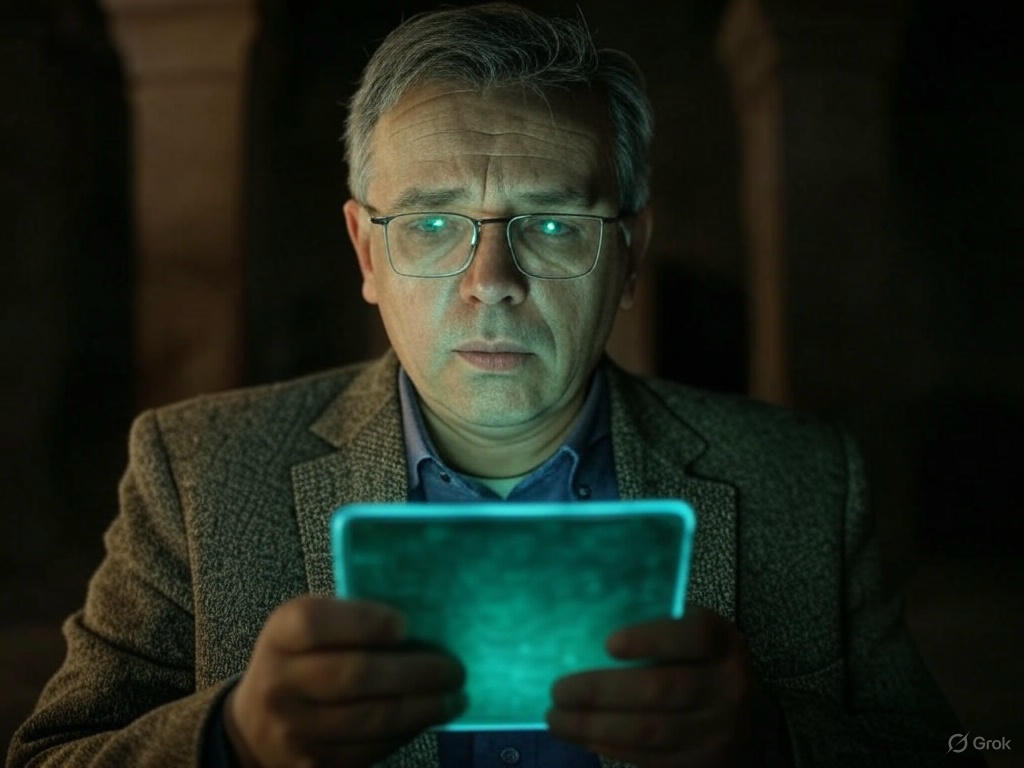
\includegraphics[width=\linewidth, height=4cm, keepaspectratio=true]{varn_picture.jpg}
            \vspace{0pt}
        \end{minipage}%
        \hspace{0.2cm}%
        \begin{minipage}[t][4cm]{0.74\linewidth}  % Adjusted height
            \centering
            % TextField with doubled font size (20pt) and increased height
            \TextField[name=character_name, width=8cm, height=2cm, multiline=true, default={Dr. Varn @AncientTechOracle}, charsize=20pt, backgroundcolor=boxcontentbg, borderwidth=0, bordercolor=boxcontentbg]{}
        \end{minipage}
    \end{tcolorbox}

    \vspace{3mm}

    % Defining the BACKGROUND box
    \begin{tcolorbox}[
        width=12.5cm,
        height=6.5cm,
        title=BACKGROUND,
        colback=boxcontentbg,
        colframe=boxborder,
        coltitle=boxheaderfg,
        colbacktitle=boxheaderbg,
        fonttitle=\bfseries\sffamily\small,
        clip upper,
        before skip=0pt
    ]
        \TextField[name=background, width=11.5cm, height=5.5cm, multiline=true, default={Former astrophysicist obsessed with ancient alien theories. With 2.3M followers on YouTube (@AncientTechOracle), he's become a leading voice in alternative archaeology. His channel, known for dramatic reveals and theatrical presentations, funds his global expeditions. Believes megalithic sites are stargates and travels the world seeking proof. Wears a tinfoil hat unironically in public. Carries a custom-made device he claims can detect ancient energies. Often speaks in cryptic pronouncements about celestial alignments and cosmic energies.}, backgroundcolor=boxcontentbg, borderwidth=0, bordercolor=boxcontentbg]{}
    \end{tcolorbox}

    \vspace{3mm}

    % Abilities box
    \begin{tcolorbox}[
        width=12.5cm,
        height=4cm,
        title=ABILITIES (choose 3),
        colback=boxcontentbg,
        colframe=boxborder,
        coltitle=boxheaderfg,
        colbacktitle=boxheaderbg,
        fonttitle=\bfseries\sffamily\small,
        clip upper,
        before skip=0pt
    ]
        \TextField[name=abilities, width=11.5cm, height=3cm, multiline=true, default={\newlinechar Ancient Tech \qquad \hspace{10mm} Social Media \newline \qquad \newline Pyramid Explorer \qquad Electrical Eng Persuasion Ste}, backgroundcolor=boxcontentbg, borderwidth=0, bordercolor=boxcontentbg]{}
    \end{tcolorbox}
\end{minipage}
\hfill
\begin{minipage}[t]{0.48\textwidth}
    \vspace{0pt}
    % Sanity box
    \begin{tcolorbox}[
        width=12.5cm,
        height=2.5cm,
        title=SANITY,
        colback=boxcontentbg,
        colframe=boxborder,
        coltitle=boxheaderfg,
        colbacktitle=boxheaderbg,
        fonttitle=\bfseries\sffamily\small,
        clip upper,
        before skip=0pt
    ]
        \begin{minipage}[t]{\linewidth}
            \large \hspace*{2mm}
            $\bigcirc$ \hspace{1em}
            $\bigcirc$ \hspace{1em}
            $\bigcirc$ \hspace{1em}
            $\bigcirc$ \hspace{1em}
            $\bigcirc$ \hspace{1em}
            $\bigcirc$ \\
            \textit{\footnotesize \hspace*{2mm} (6 = Sanity breaks)} \\
            \vspace{2mm}
            \textit{\footnotesize \hspace*{2mm} Check one circle each time sanity decreases.}
        \end{minipage}
    \end{tcolorbox}

    \vspace{3mm}

    % Personality box
    \begin{tcolorbox}[
        width=12.5cm,
        height=3.5cm,
        title=PERSONALITY (choose 2),
        colback=boxcontentbg,
        colframe=boxborder,
        coltitle=boxheaderfg,
        colbacktitle=boxheaderbg,
        fonttitle=\bfseries\sffamily\small,
        clip upper,
        before skip=0pt
    ]
        \TextField[name=personality, width=11.5cm, height=2.5cm, multiline=true, default={Adventurous	 Analytical 	Charismatic 	Cautious Obsessive}, backgroundcolor=boxcontentbg, borderwidth=0, bordercolor=boxcontentbg]{}
    \end{tcolorbox}

    \vspace{3mm}

    % Handicaps box
    \begin{tcolorbox}[
        width=12.5cm,
        height=3.5cm,
        title=HANDICAPS (choose 2),
        colback=boxcontentbg,
        colframe=boxborder,
        coltitle=boxheaderfg,
        colbacktitle=boxheaderbg,
        fonttitle=\bfseries\sffamily\small,
        clip upper,
        before skip=0pt
    ]
        \TextField[name=handicaps, width=11.5cm, height=2.5cm, multiline=true, default={Claustrophobia Dust Allergy Technophobia Night Blindness Driven by Visions}, backgroundcolor=boxcontentbg, borderwidth=0, bordercolor=boxcontentbg]{}
    \end{tcolorbox}

    \vspace{3mm}

    % Equipment box
    \begin{tcolorbox}[
        width=12.5cm,
        height=5cm,
        title=EQUIPMENT (choose 4),
        colback=boxcontentbg,
        colframe=boxborder,
        coltitle=boxheaderfg,
        colbacktitle=boxheaderbg,
        fonttitle=\bfseries\sffamily\small,
        clip upper,
        before skip=0pt
    ]
        \TextField[name=equipment, width=11.5cm, height=4cm, multiline=true, default={Power Generator  Sat Comm  EMF Detector  Night Goggles  Digging Tools  Smartphone  Smoke Grenades  First Aid  Mushrooms  Snubnose Revolver}, backgroundcolor=boxcontentbg, borderwidth=0, bordercolor=boxcontentbg]{}
    \end{tcolorbox}
\end{minipage}

% End of the form
\end{Form}

\end{document}